\chapter{Introduction into bacterial interactions}
Interactions in natural microbial communities are a very common phenomenon~\cite{Weiland-Brauer2021-eq, Braga2016-fr}, yet replicating such communities in a controlled environment is challenging~\cite{Oriano2020-ro}, and therefore the impact of such interactions on single species or whole communities is often overlooked~\cite{Virgo2025-zv}. Interactions can be very diverse in their type and range from very simple ones, such as resource competition, limiting the growth of other members of the community due to the absence of a critical resource~\cite{Ghoul2016-qx, Bakkeren2025-fv}, to highly complex interactions, involving multiple partners and toxin production~\cite{Kerr2002-ny, Wright2016-bs}. These interactions can have synergistic~\cite{Sarsan2021-pn}, symbiotic~\cite{Pawlowska2024-go} or antagonistic effects~\cite{Feichtmayer2017-lv}. In this thesis, we focus on antagonistic interactions. These are interactions where one interaction partner harms the other's growth to gain a benefit itself. In this thesis, we study two of the most well-known antagonistic interactions in two different projects. In the first project, we investigate antibiotic production \textit{in vitro}. Antibiotics or antimicrobial compounds are toxins produced by various microorganisms to harm nearby competitors, as sketched in Figure~\ref{fig:intro_shared_interactions}, upper part. These competitors can evolve resistance to the toxin and possibly antibiotic producers can modify their toxin production through evolution in a so-called arms race. Our work studies a possible way to select and evolve antibiotic production. The second project investigates \gls{phage} infection using computational modeling. Phages are viruses that infect bacteria and as such play a vital role in natural communities. However, little is known about the interactions between bacteria and phages when populating a new environment. In this project, we focus on the impact of resource competition on these interactions (Figure~\ref{fig:intro_shared_interactions}, lower part).

\begin{figure}
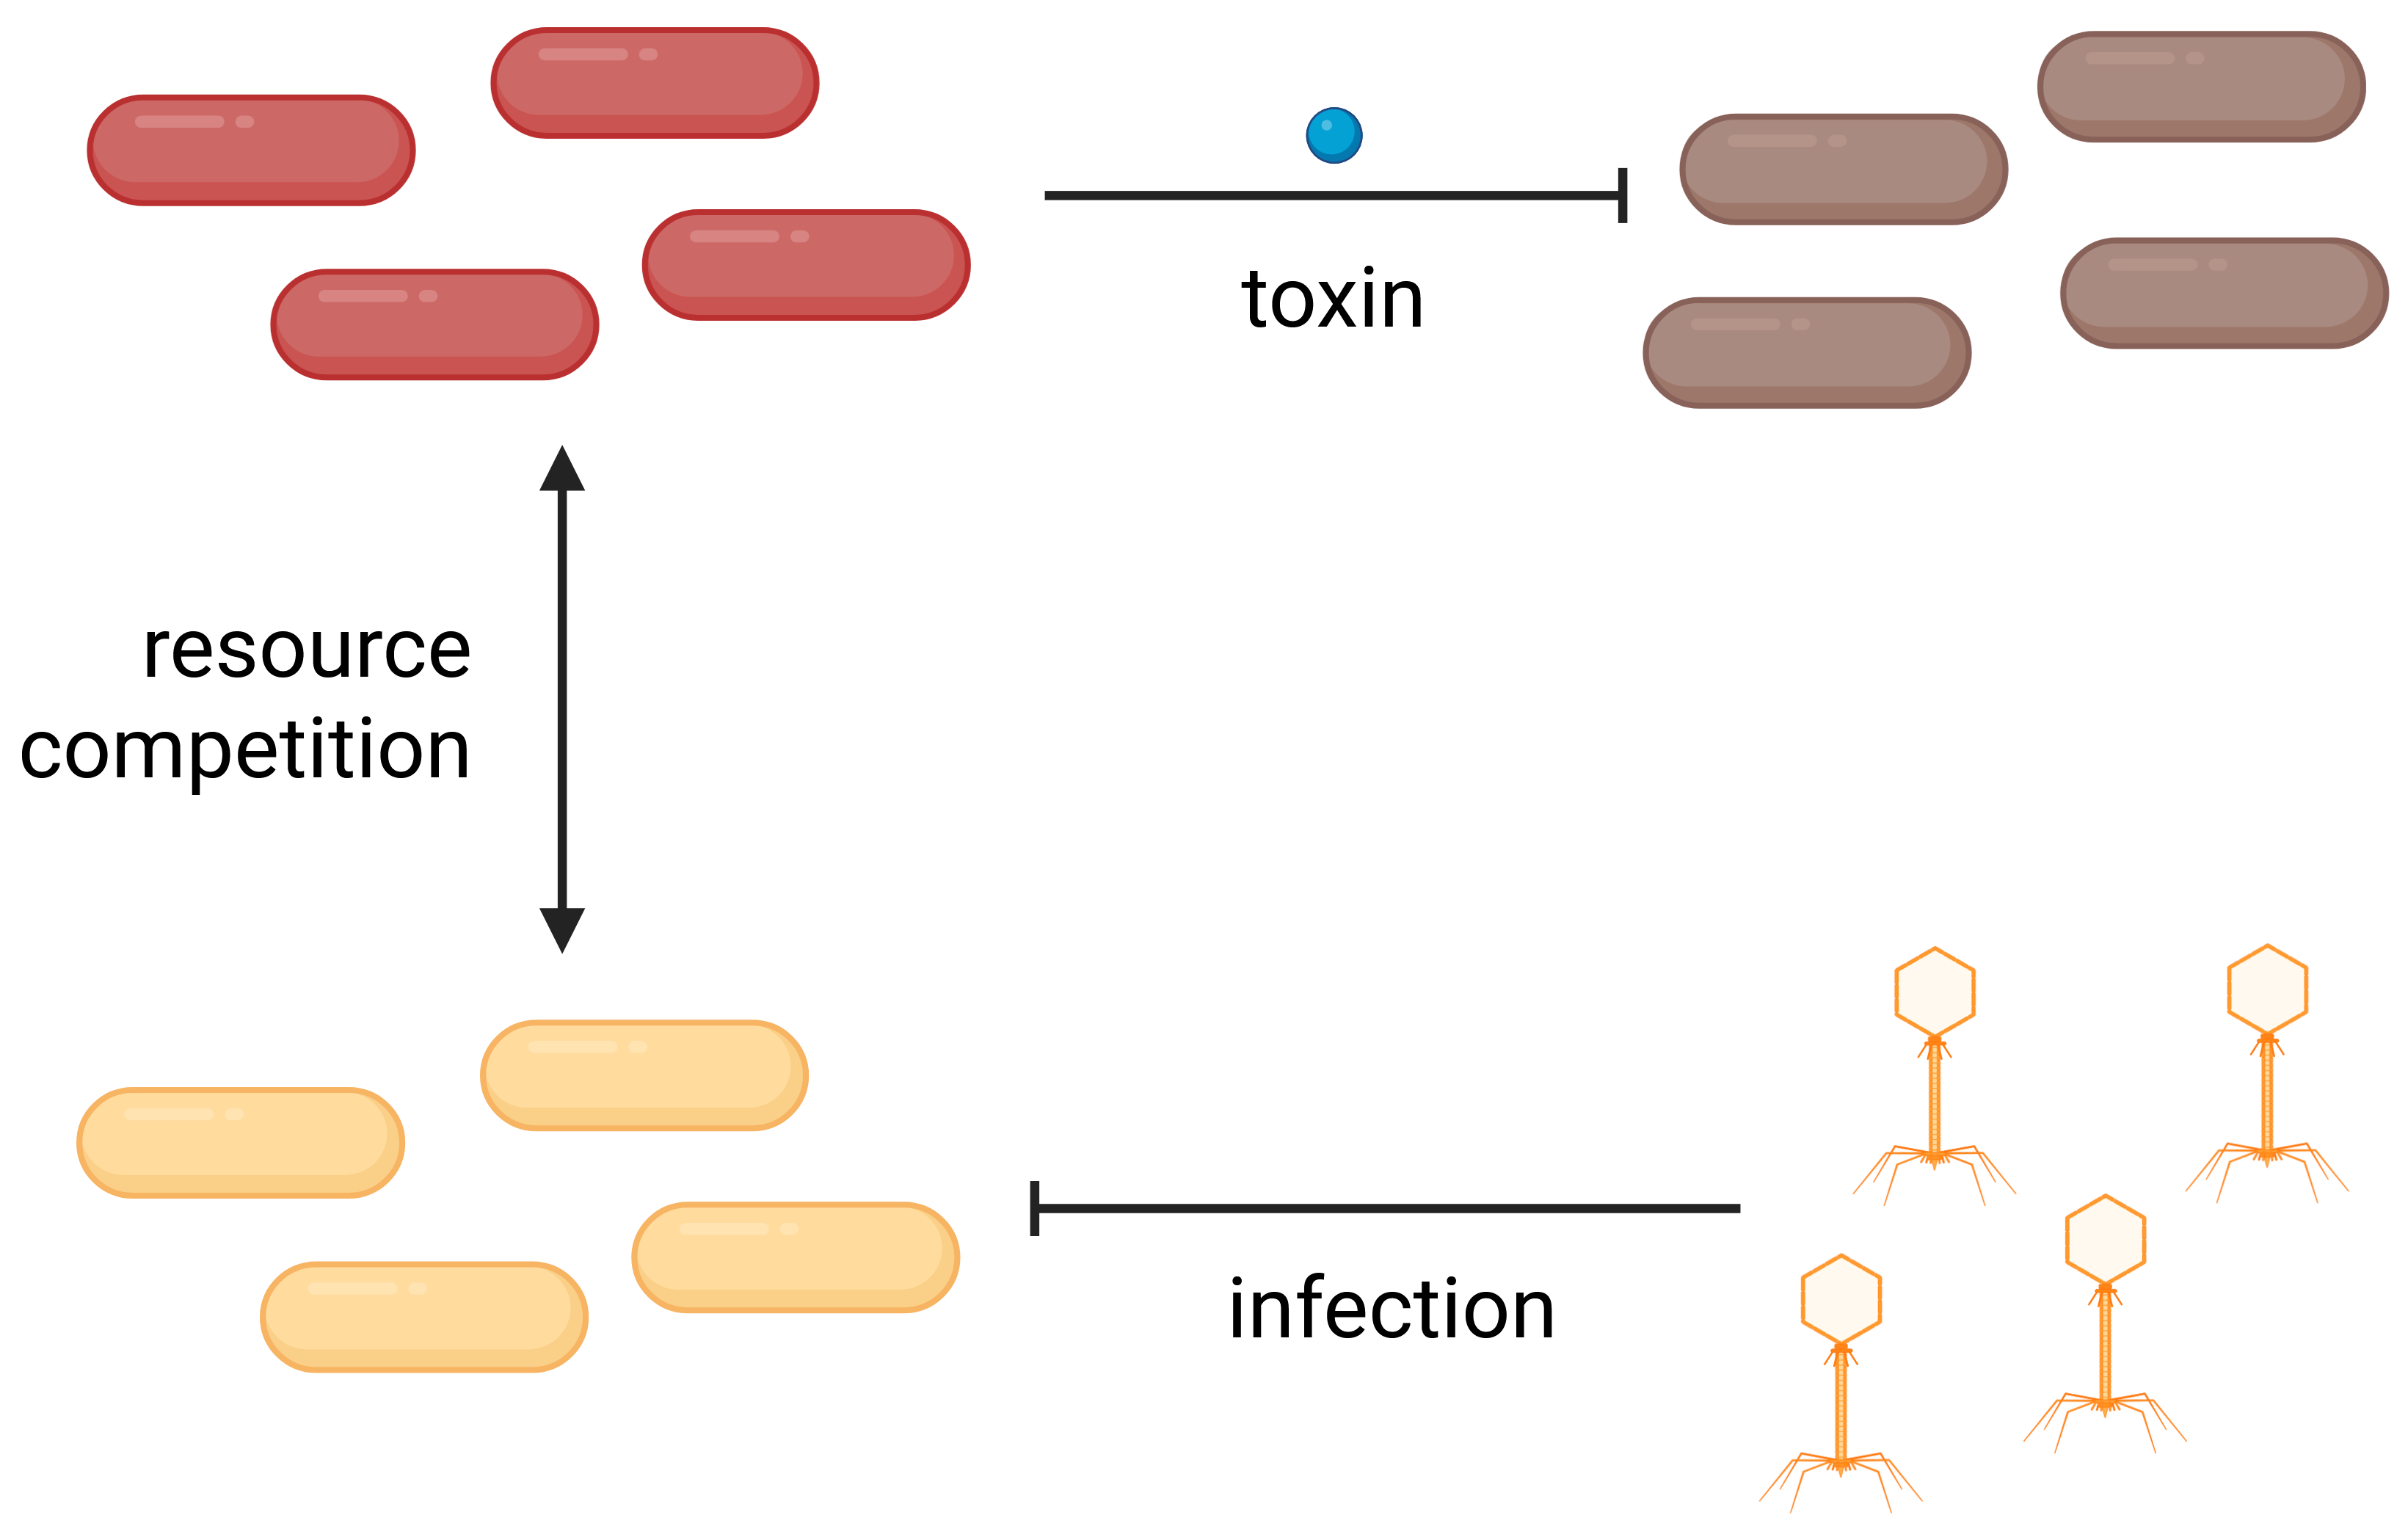
\includegraphics[width=\linewidth]{graphics/2025_09_30_intro_fig1.png}
\caption{\textbf{Antibiotic production and phage infection are common, antagonistic interactions studied in this thesis} The sketch shows two common, antagonistic interactions in microbial communities. The upper part of the sketch shows the production of a toxin (blue) by a bacterial strain (red) which can then inhibit another target strain (brown), sensitive to the produced toxin. At the same time there are other, resistant, members in the community (yellow) which compete for available resources but are not inhibited by the toxin. This interaction will be studied in the first, experimental project of this thesis. The lower part of the sketch shows the infection of a bacterial species by \gls{phage}s, viruses which infect bacteria. Phage infections form an integral, important part of natural ecology. In addition to phage infection, the phage-sensitive bacteria are in resource competition with phage-resistant bacteria. This bacteria-phage interaction will be studied in the second, theoretical project of this thesis in a spatially structured environment.}
\label{fig:intro_shared_interactions}
\end{figure}